% Micromechanics with MMM: from the bubble case to the pore population, first RVE tests
% E. Cappellari -- update for T. Barani, 27 October 2026
% Build: latexmk -pdf mmm_polydisperse.tex      Figures in mmm_polydisperse_figs/ (plot_bubbles.py, mm-opera-hpc)

\documentclass[10pt,aspectratio=169]{beamer}
\usepackage[T1]{fontenc}
\usepackage[utf8]{inputenc}
\usepackage{lmodern}
\usepackage{amsmath,amssymb,booktabs,graphicx,tikz,array}
\usetikzlibrary{arrows.meta,positioning}
\graphicspath{{mmm_polydisperse_figs/}}

% ---- plain white style ------------------------------------------------------------------------------------------------
\usefonttheme[onlymath]{serif}
\setbeamertemplate{navigation symbols}{}
\setbeamercolor{background canvas}{bg=white}
\setbeamercolor{normal text}{fg=black}
\setbeamercolor{structure}{fg=black!75}
\setbeamercolor{frametitle}{fg=black}
\setbeamercolor{title}{fg=black}
\setbeamercolor{subtitle}{fg=black!70}
\setbeamerfont{frametitle}{size=\Large,series=\bfseries}
\setbeamerfont{title}{size=\LARGE,series=\bfseries}
\setbeamertemplate{itemize items}[circle]
\setbeamertemplate{enumerate items}[default]
\setbeamertemplate{footline}{\hfill{\color{black!45}\scriptsize\insertframenumber/\inserttotalframenumber}\hspace{5mm}\vspace{3mm}}
\setbeamertemplate{caption}{\raggedright\insertcaption\par}
\setlength{\abovedisplayskip}{4pt}
\setlength{\belowdisplayskip}{4pt}

% ---- colour code of the previous updates ---------------------------------------------------------------------------
\definecolor{paper}{RGB}{0,80,180}
\definecolor{own}{RGB}{190,50,40}
\newcommand{\pp}[1]{{\color{paper}#1}}   % from a paper / OperaHPC D5.2
\newcommand{\oo}[1]{{\color{own}#1}}     % our own choice
\newcommand{\sI}{\sigma_I^{\max}\big|_i}
\newcommand{\code}[1]{\texttt{#1}}

\title{How Fission Gas Pressurised Pores Drive High Burnup Fuel Fragmentation:\\ A Micromechanics-Informed Pore Population Model in SCIANTIX}
\author{E.\ Cappellari}
\date{27 October 2026}

\begin{document}

{\setbeamertemplate{footline}{}
\begin{frame}
\titlepage
\end{frame}}

% ---------------------------------------------------------------------------------------------------------------------
\begin{frame}{Outline}
\centering
\resizebox{\linewidth}{!}{%
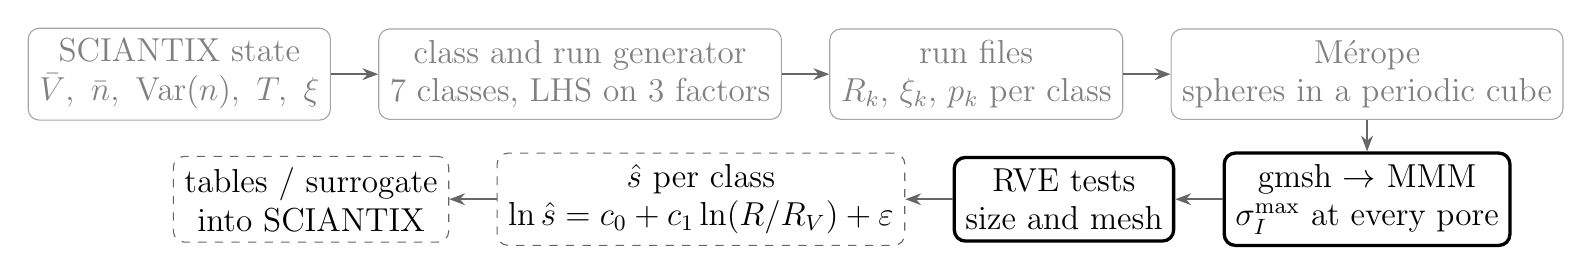
\begin{tikzpicture}[node distance=4mm and 6mm, every node/.style={font=\large},
  box/.style={draw, rounded corners, align=center, minimum height=9mm, inner sep=4pt},
  done/.style={box, draw=black!35, text=black!50},
  new/.style={box, very thick},
  next/.style={box, dashed, draw=black!60},
  arr/.style={-{Stealth[length=2mm]}, thick, black!60}]
\node[done] (sx) {SCIANTIX state\\ $\bar V,\ \bar n,\ \mathrm{Var}(n),\ T,\ \xi$};
\node[done, right=of sx] (pd) {class and run generator\\ 7 classes, LHS on 3 factors};
\node[done, right=of pd] (rf) {run files\\ $R_k$, $\xi_k$, $p_k$ per class};
\node[done, right=of rf] (me) {M\'erope\\ spheres in a periodic cube};
\node[new, below=of me] (gm) {gmsh $\to$ MMM\\ $\sigma_I^{\max}$ at every pore};
\node[new, left=of gm] (rve) {RVE tests\\ size and mesh};
\node[next, left=of rve] (fit) {$\hat s$ per class\\ $\ln\hat s=c_0+c_1\ln(R/R_V)+\varepsilon$};
\node[next, left=of fit] (tab) {tables / surrogate\\ into SCIANTIX};
\draw[arr] (sx) -- (pd); \draw[arr] (pd) -- (rf); \draw[arr] (rf) -- (me); \draw[arr] (me) -- (gm);
\draw[arr] (gm) -- (rve); \draw[arr] (rve) -- (fit); \draw[arr] (fit) -- (tab);
\end{tikzpicture}}
\vspace{8pt}

\small\raggedright\begin{itemize}\small
\item \code{bubble} case of mm-opera-hpc adapted to a population of pores: \code{polydispersebubble}
\item pipeline M\'erope $\to$ gmsh $\to$ MMM $\to$ analysis, first size and mesh tests on 10 cubes
\end{itemize}
\end{frame}

% ---------------------------------------------------------------------------------------------------------------------
\begin{frame}{Starting point: \code{bubble} (OperaHPC D5.2)}

Elastic matrix $\Omega_m$ around pressurised pores, periodic cube:
\[
\nabla\cdot\boldsymbol\sigma=\mathbf 0,\qquad \boldsymbol\sigma=\mathbb C:\boldsymbol\varepsilon(\mathbf u)\quad\text{in }\Omega_m
\]
\[
\boldsymbol\sigma\,\mathbf n=-p\,\mathbf n\ \text{ on the pores},\qquad
\mathbf u-\langle\boldsymbol\varepsilon\rangle\mathbf x\ \text{periodic},\quad \langle\boldsymbol\varepsilon\rangle=\mathbf 0
\]
$E=150$ GPa, $\nu=0.3$, lengths in $\mu$m.
\[
p_{hyd}=-\tfrac13\,\mathrm{tr}\Bigl(\tfrac1V\textstyle\int_V\boldsymbol\sigma\,dV\Bigr).
\]

Rupture and release
\[
\sI=\max_{|\mathbf x-\mathbf c_i|\le d_{min}}\sigma_I(\mathbf x),\qquad
\mathrm{FGR}=\frac{\sum_i V_i\,\bigl[\sI(p)>\sigma_R\bigr]}{\sum_i V_i}
\]
\end{frame}

% ---------------------------------------------------------------------------------------------------------------------
\begin{frame}{From \code{bubble} to \code{polydispersebubble}}
\renewcommand{\arraystretch}{1.25}
\begin{tabular}{@{}>{\raggedright\arraybackslash}p{0.17\linewidth}>{\raggedright\arraybackslash}p{0.27\linewidth}>{\raggedright\arraybackslash}p{0.50\linewidth}@{}}
\toprule
 & \code{bubble} & \code{polydispersebubble}\\
\midrule
pressure & one $p$ for all the pores & one pressure per pore: $\boldsymbol\sigma\mathbf n=-p_{ref}\,p_i\,\mathbf n$ on pore $i$ (6th column of the pore list) \\
search sphere & fixed $d_{min}=0.95\ \mu$m from the centre; pore of $R=0.4\ \mu$m: shell of 0.55 $\mu$m & $R_i+\delta$, here $\delta=0.5\ \mu$m: the same shell for every pore size\\
pores evaluated & near the global maximum ($\sigma_I>0.9\max$) & all the pores: the FGR needs $\sI$ of every pore \\
output & points, \code{id x y z stress} & id, R, p, $\sigma_I^{\max}$, x, y, z; $\langle\sigma_h\rangle$, for every pore \\
\bottomrule
\end{tabular}
\vspace{8pt}
\[
\sI=\max_{\mathbf x\in\Omega_m,\ |\mathbf x-\mathbf c_i|\le R_i+\delta}\ \sigma_I(\mathbf x)
\]
\end{frame}

% ---------------------------------------------------------------------------------------------------------------------
\begin{frame}{Numerical and HPC choices}
\begin{columns}[T]
\column{0.5\linewidth}
\textbf{Solver}
\begin{itemize} 
\item Preconditioned conjugate gradient, the iterative solver of $K\mathbf u=\mathbf f$: BoomerAMG instead of the diagonal one. The diagonal one only rescales every equation: the iterations grow as the mesh is refined. AMG also corrects the error on coarser levels built from $K$: the iterations stay almost constant with the mesh size
\item single-pore case: 100 * iterations with the diagonal one with respect to BoomerAMG;
\item maximum number of iterations raised from 1000 to 5000 as a margin for the larger meshes
\end{itemize}
\column{0.5\linewidth}
\textbf{Memory and MPI}
\begin{itemize} 
\item every rank searches only its own maximum stress point for each bubble, then one gather of $[\sigma,x,y,z]\times n_{pores}$:
      exact global maximum per pore
\item the original copied all the points on every rank: hundreds of millions with all the pores
\end{itemize}
\vspace{6pt}
\textbf{Outputs}
\begin{itemize} 
\item pore list and $\langle\sigma_h\rangle$ always; ParaView fields on request
\end{itemize}
\end{columns}
\end{frame}

% ---------------------------------------------------------------------------------------------------------------------
\begin{frame}{From the MMM run to the rupture criterion}

Runs at unit pressure in every pore, zero macroscopic strain. Per pore $\sigma_i=\sI/p$, and the mean hydrostatic
stress of the matrix $\langle\sigma_h\rangle$ ($<0$).
\vspace{4pt}

\textbf{Back to zero macroscopic stress} (superposition $\boldsymbol\sigma(p-p_{hyd},0)=\boldsymbol\sigma(p,p_{hyd})+p_{hyd}\mathbf I$):
\[
h=\frac{p_{hyd}}{p}=\xi-(1-\xi)\,\frac{\langle\sigma_h\rangle}{p},\qquad
\hat s_i=\frac{\sigma_i+h}{1-h}
\]
exact when all the pores have the same pressure.
\vspace{4pt}

\textbf{Rupture and release}: pore $i$ breaks when $\hat s_i\,p>\sigma_R$, i.e.\ at $x_{c,i}=1/\hat s_i$ with $x=p/\sigma_R$:
\[
\mathrm{FGR}(x)=\frac{\sum_i V_i\,\mathbf 1\bigl[\hat s_i\,x>1\bigr]}{\sum_i V_i}
\]
One MMM run gives the whole curve, for any $\sigma_R$.
\end{frame}

% ---------------------------------------------------------------------------------------------------------------------
\begin{frame}[fragile]{Pipeline}
\centering
\resizebox{\linewidth}{!}{%
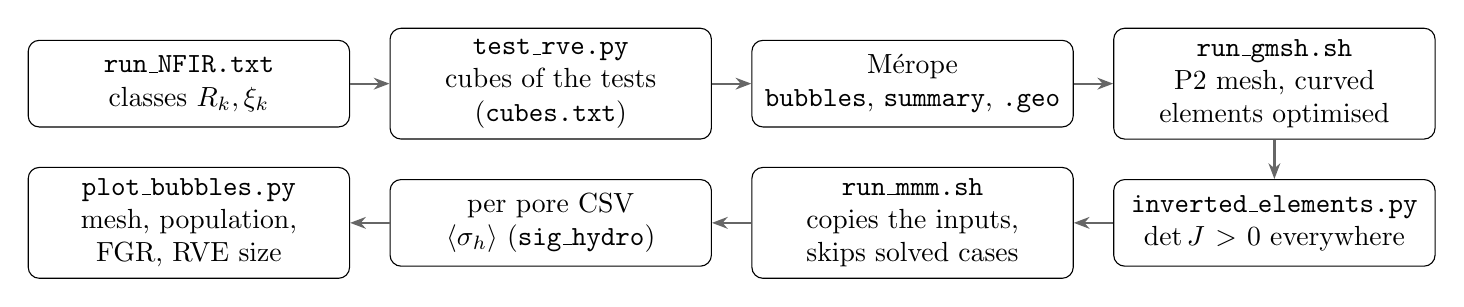
\begin{tikzpicture}[node distance=5mm and 5mm, every node/.style={font=\normalsize},
  box/.style={draw, rounded corners, align=center, minimum height=11mm, inner sep=4pt, text width=38mm},
  arr/.style={-{Stealth[length=2mm]}, thick, black!60}]
\node[box] (run) {\texttt{run\_NFIR.txt}\\ classes $R_k,\xi_k$};
\node[box, right=of run] (cub) {\texttt{test\_rve.py}\\ cubes of the tests\\ (\texttt{cubes.txt})};
\node[box, right=of cub] (mer) {M\'erope\\ \texttt{bubbles}, \texttt{summary}, \texttt{.geo}};
\node[box, right=of mer] (gm) {\texttt{run\_gmsh.sh}\\ P2 mesh, curved\\ elements optimised};
\node[box, below=of gm] (chk) {\texttt{inverted\_elements.py}\\ $\det J>0$ everywhere};
\node[box, left=of chk] (mmm) {\texttt{run\_mmm.sh}\\ copies the inputs,\\ skips solved cases};
\node[box, left=of mmm] (out) {per pore CSV\\ $\langle\sigma_h\rangle$ (\texttt{sig\_hydro})};
\node[box, left=of out] (ana) {\texttt{plot\_bubbles.py}\\ mesh, population,\\ FGR, RVE size};
\draw[arr] (run) -- (cub); \draw[arr] (cub) -- (mer); \draw[arr] (mer) -- (gm); \draw[arr] (gm) -- (chk);
\draw[arr] (chk) -- (mmm); \draw[arr] (mmm) -- (out); \draw[arr] (out) -- (ana);
\end{tikzpicture}}
\vspace{6pt}

\begin{columns}[T]
\column{0.48\linewidth}
\scriptsize
\begin{verbatim}
test_rve_side10/run_NFIR/
  side10_seed01 ... side10_seed10      size test
  side10_seed01_meshdouble             mesh test
  side10_seed01_meshdouble_refinement  refined in MMM
  cubes.txt  unit_NFIR.txt
\end{verbatim}
\column{0.48\linewidth}
\begin{itemize}
\item one folder per cube: pore list, summary, mesh, MMM outputs
\item the folder name tells the analysis what the cube is (side, seed, variant)
\end{itemize}
\end{columns}
\end{frame}

% ---------------------------------------------------------------------------------------------------------------------
\begin{frame}{Data analysis}
\begin{enumerate}
\item \textbf{Is the mesh fine enough?} Class means of $\hat s$ on a coarser mesh against the finest one, tolerance 2 \%.
\item \textbf{Does a cube hold the whole population?} Pores expected and placed per class: a class with less than one
      pore per cube is missing from every cube, whatever the number of seeds.
\item \textbf{How much does the FGR change between seeds?} $x_c=p/\sigma_R$ at which every cube releases 10, 25, 50, 75,
      90 \% of the gas, compared between the 10 cubes.
\item \textbf{Which side gives the precision asked?} Kanit's method (next slide) on $x_c$ and on the class means of
      $\hat s$.
\end{enumerate}
 
\end{frame}

% ---------------------------------------------------------------------------------------------------------------------
\begin{frame}{Size of the RVE: the method of Kanit et al.\ 2003}
\begin{columns}[T]
\column{0.47\linewidth}
\small
\textbf{Quantities}, for one class of pores:
\begin{itemize}
\item $Z$: mean of $\hat s$ over the pores of the class in \emph{one} cube (one value per cube)
\item $\bar Z$: mean of $Z$ over the $n=10$ cubes (seeds)
\item $D^2$: variance of $Z$ between the cubes
\item $S^2$: variance of $\hat s$ between single pores
\item $V=L^3$: volume of the cube
\item $A$: integral range, the volume over which $\hat s$ is correlated; for independent pores $A=1/$(pore density) [HOW IS CALCULATED?]
\item $\alpha$: how fast the spread falls with the volume; $\alpha=1$ for independent pores (variance of a mean of $N$
      values $=S^2/N$) [NON CAPISCO come lo calcoli]
\end{itemize}
\column{0.5\linewidth}
\footnotesize
Spread between cubes and error of one cube (95 \%):
\[
D^2(V)=S^2\Bigl(\frac{A}{V}\Bigr)^{\alpha},\qquad
\varepsilon_{cube}=\frac{2D}{\bar Z}
\]
One cube is an RVE if $\varepsilon_{cube}\le\varepsilon_R=5\ \%$. Otherwise, with $\alpha=1$:
\[
n=\Bigl(\frac{\varepsilon_{cube}}{\varepsilon_R}\Bigr)^{2}\ \text{cubes of side }L,
\]
or one cube of side
\[
L_{RVE}=L\Bigl(\frac{\varepsilon_{cube}}{\varepsilon_R}\Bigr)^{2/3}
\]
$D^2$ comes from only 10 cubes: its 95 \% confidence interval ($\chi^2$ distribution, 9 degrees of freedom) gives the
range of $L_{RVE}$ written next to it, e.g.\ 27 $\mu$m (21--40).
\vspace{4pt}

Check of $\alpha=1$: independent pores give $A\times\text{density}=D^2N_k/S^2=1$ ($N_k$ pores of the class per cube).
\end{columns}
\end{frame}

% ---------------------------------------------------------------------------------------------------------------------
\begin{frame}{Test set-up and cost}
\begin{columns}[T]
\column{0.5\linewidth}
\small
\textbf{Pores}: NFIR disc before the anneal, 7 classes $R=0.22$--$1.70\ \mu$m, $\xi=0.114$, $R_V=0.73\ \mu$m;
unit pressure in every pore; repulsion 0.3 $\mu$m; $\delta=0.5\ \mu$m.
\vspace{6pt}

\textbf{Cubes}: 10 cubes of 10 $\mu$m at mesh 0.3 $\mu$m (size test) + seed 1 at 0.6 $\mu$m (mesh test).
\vspace{6pt}

\textbf{Planned}: 30 $\mu$m at 0.15 $\mu$m, but on the cluster (should be available now).
\column{0.46\linewidth}
\small
\textbf{Does a 10 $\mu$m cube hold the population?}
\begin{center}
\footnotesize
\begin{tabular}{@{}rrrr@{}}
\toprule
$R$ ($\mu$m) & pore vol. & expected & placed \\
\midrule
1.70 & 7.8 \% & 0.4 & \textbf{0} \\
1.19 & 26.2 \% & 4.2 & 4 \\
0.85 & 38.2 \% & 16.7 & 16 \\
0.61 & 22.2 \% & 26.5 & 26 \\
0.44 & 5.1 \% & 16.7 & 16 \\
0.31 & 0.5 \% & 4.2 & 4 \\
0.22 & 0.02 \% & 0.4 & \textbf{0} \\
\bottomrule
\end{tabular}
\end{center}
porosity 0.101 against 0.114: the 1.70 $\mu$m class needs a side $\ge13.6\ \mu$m.
\end{columns}
\end{frame}

% ---------------------------------------------------------------------------------------------------------------------
\begin{frame}{Result: FGR of the 10 cubes}
\centering
\includegraphics[width=0.94\linewidth]{rve_fgr.png}
% TODO: add the FGR curve of OperaHPC D5.2 (Fig. 7) on the same figure: needs its data (csv), not on this PC [digitalizza da deliverablde opera]
\vspace{2pt}

\raggedright\small
\begin{itemize}
\item $x_c=p/\sigma_R$ at which a cube releases 50 \% of its gas: $0.747\pm0.029$ (mean of the 10 cubes, 95 \%), i.e.\
      $p\approx205$ MPa with the $\sigma_R=275$ MPa of OperaHPC (to recalibrate)
\item error of one cube on $x_c$: 7--12 \%, above the 5 \% asked. On the FGR alone the RVE is $\approx18\ \mu$m;
      14--27 $\mu$m is its 95 \% confidence interval (only 10 cubes)
\end{itemize}
\end{frame}

% ---------------------------------------------------------------------------------------------------------------------
\begin{frame}{Result: size of the RVE}
\centering
\includegraphics[width=\linewidth]{rve_size.png}
\vspace{2pt}

\raggedright\small
\begin{itemize}
\item \textbf{one 10 $\mu$m cube is not an RVE}: $L_{RVE}\approx27\ \mu$m (21--40), set by the 1.19 $\mu$m class (26 \% of the
      pore volume), or the mean of 20 cubes of 10 $\mu$m; consistent with the 30 $\mu$m of OPERAHPC
\item is the $1/V$ scaling right? If the pores of a class act independently, $A\times$density $=1$. Measured 0.56--1.18,
      close to 1: extrapolating from 10 $\mu$m to $L_{RVE}$ with $\alpha=1$ is reasonable; a second cube side would
      measure $\alpha$ directly [TBD]
\item $\hat s$ follows the nearest ligament: it grows when the gap to the nearest pore shrinks
\end{itemize}
\end{frame}

% ---------------------------------------------------------------------------------------------------------------------
\begin{frame}{Mesh convergence (seed 1, preliminary)}
\centering
\includegraphics[width=0.86\linewidth]{mesh_test.png}
\vspace{2pt}

\raggedright\footnotesize
Same pores of seed 1 meshed at 0.6 and 0.3 $\mu$m. Left: class mean of $\hat s$ on 0.6 $\mu$m minus that on 0.3 $\mu$m,
in \% of the latter (grey band: $\pm2$ \% tolerance). Right: the same pore by pore, against the gap to the nearest pore.
\begin{itemize}
\item the classes $\ge0.85\ \mu$m ($\approx70$ \% of the pore volume) change by $\le1$ \%; the small ones by up to 35 \%
\item why it is not conclusive: with two meshes the reference (0.3 $\mu$m) is itself not converged.
\item to redo with the mesh of the final runs: 0.15 $\mu$m
\end{itemize}
\end{frame}

% ---------------------------------------------------------------------------------------------------------------------
\begin{frame}{A pitfall of curved elements: inverted tetrahedra}
\small
A P2 tetrahedron is the image of a reference one through its 10 nodes; gmsh moves the mid-edge nodes onto the sphere so
that the faces follow the pore:
\[
\mathbf x(\boldsymbol\xi)=\sum_{a=1}^{10}\mathbf x_a N_a(\boldsymbol\xi),\qquad
J=\frac{\partial\mathbf x}{\partial\boldsymbol\xi}
\]
In a thin ligament between close pores (gap $\approx$ mesh size) the curved element folds over: $\det J<0$ in part of it
and the stiffness matrix may lose positive definiteness.
\vspace{4pt}

gmsh log: {\footnotesize\code{Volume mesh: worst distortion = -15.9 (\dots, 8 elements with jac. < 0)}}\\
MMM: {\footnotesize\code{solve: the non linear solver did not converge}}
\begin{itemize}
\item 9 of 10 seeds (worst distortion $-16$ to $-18$): the linear solver fails
\item seed 1 (worst $-1.8$) converged, but its 7 inverted elements all touch the 0.31 $\mu$m pores:
      $\sigma_I^{\max}/p\approx1.65$ instead of $\approx0.59$ on three of them
\end{itemize}
\textbf{Fix}: gmsh \code{Mesh.HighOrderOptimize 2}.
\end{frame}

% ---------------------------------------------------------------------------------------------------------------------
\begin{frame}{Next steps and points to discuss}
\begin{columns}[T]
\column{0.48\linewidth}
\textbf{Next}
\begin{enumerate}\small
\item mesh test at 0.15 $\mu$m on seed 1 (other PC, $\approx40$ GB)
\item a second side (20 or 30 $\mu$m) to measure $\alpha$ and the bias of the small cube; 30 $\mu$m on the cluster
      (\code{partition-mesh}: written, not yet tested in a full run)
\item fix side and mesh, then the LHS runs:
      $\ln\hat s=c_0+c_1\ln(R/R_V)+\varepsilon$ per run
\item tables / surrogate of $(c_0,c_1,\sigma_\varepsilon)$ into SCIANTIX
\end{enumerate}
\column{0.5\linewidth}
\textbf{To discuss}
\begin{itemize}\small
\item \textbf{$\delta$}: 0.5 $\mu$m in these runs, larger than the 0.3 $\mu$m minimum gap: the search sphere can reach the
      ligament of the neighbour. $\delta\le0.3\ \mu$m?
\item \textbf{pressure per class} in the LHS runs: the rescaling to zero macroscopic stress is exact only with one
      pressure; otherwise a second run (unit isotropic strain, no pressure) and a linear combination
\item \textbf{classes missing in small cubes} (1.70 $\mu$m, 7.8 \% of the pore volume): the side follows the rarest
      large class
\end{itemize}
\end{columns}
\end{frame}

\end{document}
